%% LyX 2.2.3 created this file.  For more info, see http://www.lyx.org/.
%% Do not edit unless you really know what you are doing.
\documentclass[oneside,english]{extbook}
\usepackage[T1]{fontenc}
\usepackage[latin9]{inputenc}
\usepackage{geometry}
\geometry{verbose,tmargin=25mm,bmargin=25mm,lmargin=25mm,rmargin=25mm}
\setcounter{secnumdepth}{3}
\setcounter{tocdepth}{3}
\setlength{\parindent}{0bp}
\synctex=1
\usepackage{babel}
\usepackage{float}
\usepackage{graphicx}
\usepackage{setspace}
\usepackage{subscript}
\onehalfspacing
\usepackage[unicode=true,pdfusetitle,
 bookmarks=true,bookmarksnumbered=false,bookmarksopen=false,
 breaklinks=false,pdfborder={0 0 1},backref=false,colorlinks=false]
 {hyperref}

\makeatletter
%%%%%%%%%%%%%%%%%%%%%%%%%%%%%% User specified LaTeX commands.
\usepackage{color}
\usepackage{listings}
\usepackage{pdflscape}
\definecolor{hellgelb}{rgb}{1,1,0.85}
\definecolor{colKeys}{rgb}{0,0,1}
\definecolor{colIdentifier}{rgb}{0,0,0}
\definecolor{colComments}{rgb}{1,0,0}
\definecolor{colString}{rgb}{0,0.5,0}
\lstset{
      language=Matlab,
      float=hbp,
      basicstyle=\footnotesize\ttfamily,
      identifierstyle=\color{colIdentifier},
      keywordstyle=\color{colKeys},
      stringstyle=\color{colString},
      commentstyle=\itshape\color{colComments},
      columns=fixed,
      tabsize=4,
      frame=single,
      framerule=1pt,
      extendedchars=true,
      showspaces=false,
      showstringspaces=false,
      numbers=left,
      numberstyle=\tiny\ttfamily,
      numbersep=1em,
      breaklines=true,
      breakindent=10pt,
      backgroundcolor=\color{hellgelb},
      breakautoindent=true,
      captionpos=t,
      xleftmargin=1em,
      xrightmargin=\fboxsep
}

\makeatother

\begin{document}
\pagenumbering{gobble}

We're looking for a way to get rid of those landmarks that appear
at some point in time but then are not measured subsequently and still
stay in the list of landmarks in our particles. Here is an approach
to deal with those spurious landmarks. When the robot observes a landmark
for the first time the algorithm initializes a new EKF for that landmark
and it also sets a counter to one for that landmark. If the robot
moves on and observes the same landmark for the second time the algorithm
will increment this counter by one, so the counter for that landmark
will value 2. Each time the robot observes that landmark the algorithm
increments the asocciated counter by one. This count value is a measure
of confidence for the existence of that landmark.

\begin{figure}[H]
\centering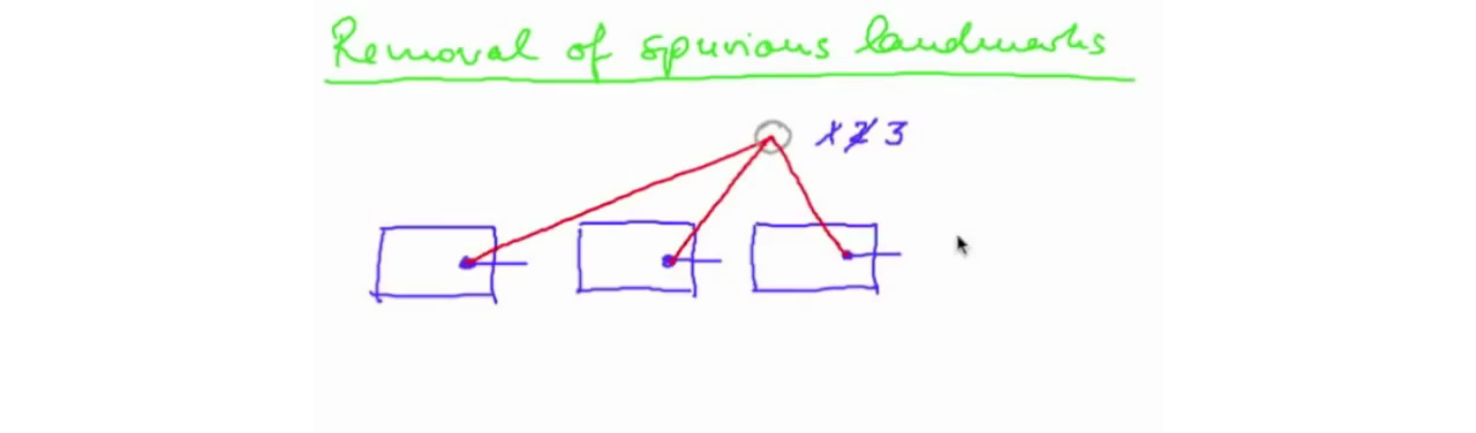
\includegraphics[scale=0.8]{../FIGURES/fig63}
\end{figure}

If the robot moves on to a place where it can't see the landmark anymore
the algorithm has to decide if it shall decrement the associated counter
for that landmark or if it shall leave the counter as is. If the algorithm
decrements the counter associated to a landmark when the robot can't
see it, then, after several movements of the robot the counter's value
would be 2, then 1, then 0 and then -1, and finally the algorithm
would remove the landmark when the counter's value is below 0.

\begin{figure}[H]
\centering\includegraphics[scale=0.8]{../FIGURES/fig64}
\end{figure}

This strategy would mean that the algorithm would forget landmarks
if it doesn't observe them regularly. This looks good at first sight,
however remember the situation in our arena. The robot starts at the
point labeled as A, then it moves and observes some landmarks for
a number of times.

\begin{figure}[H]
\centering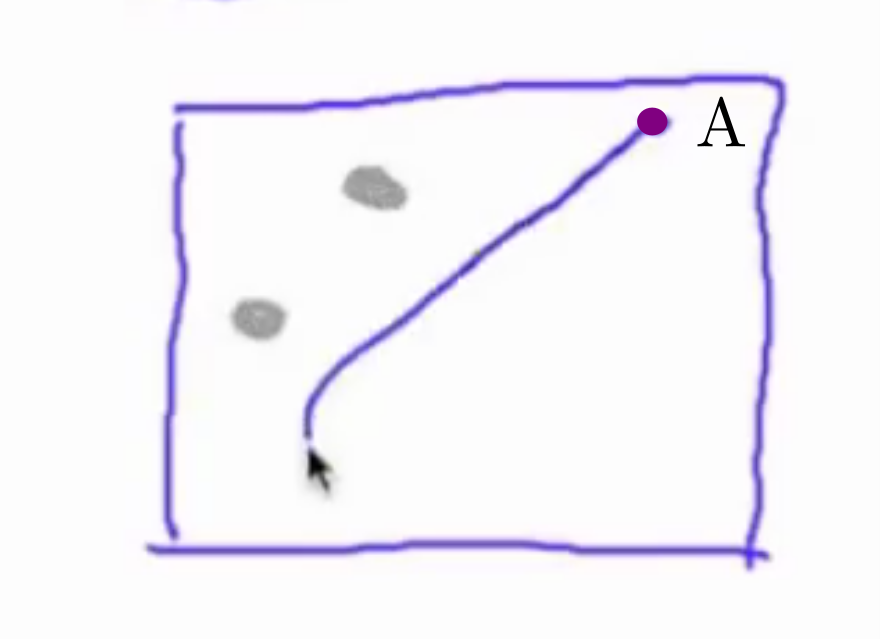
\includegraphics{../FIGURES/fig65}
\end{figure}

Whe the robot is at point B the landmarks are clearly out of sight
of the robot.

\begin{figure}[H]
\centering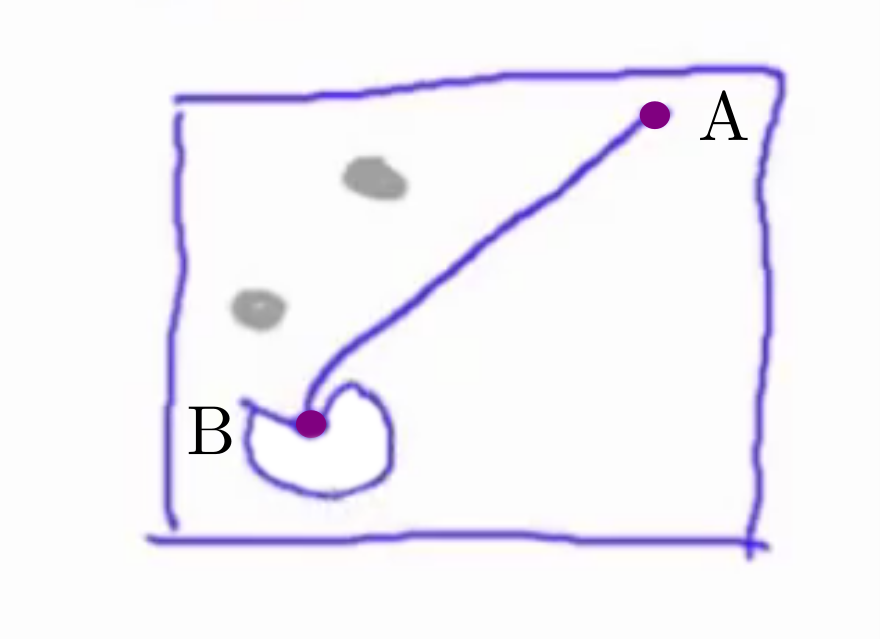
\includegraphics{../FIGURES/fig66}
\end{figure}

After a while the algorithm will forget those landmarks.

\begin{figure}[H]
\centering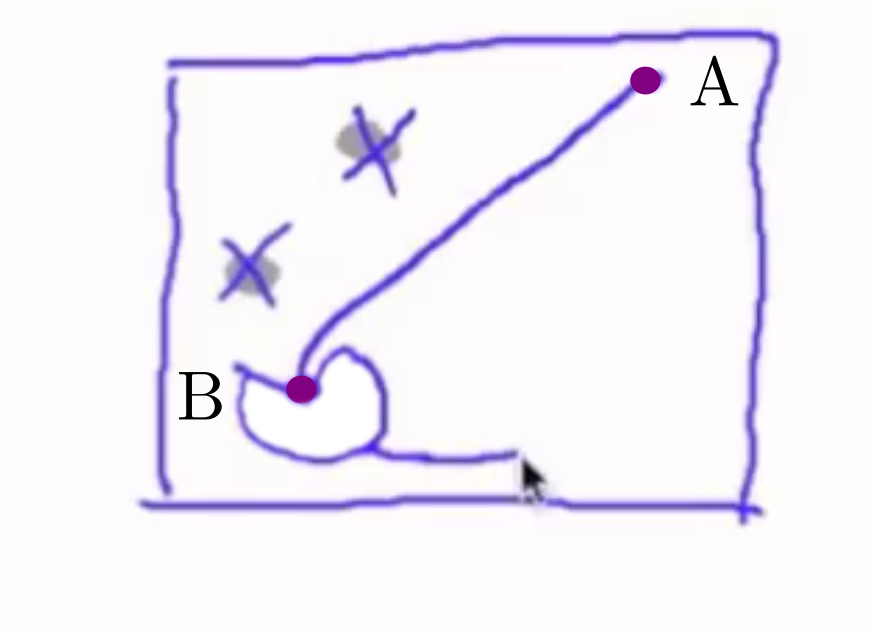
\includegraphics{../FIGURES/fig67}
\end{figure}

Later on the robot sees again the landmarks, however, at that moment
the algorithm will have forgotten them so it has to reinitialize the
landmarks and all the earlier measurements which have led to a precise
precision of the landmarks are lost.

\begin{figure}[H]
\centering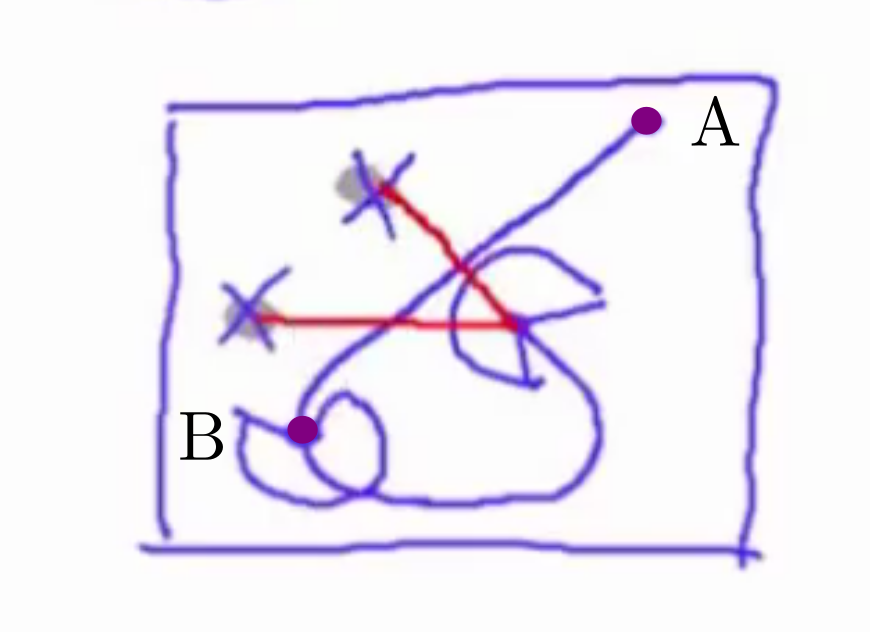
\includegraphics{../FIGURES/fig68}
\end{figure}

Therefore, we will adopt the following strategy: if our robot sees
the landmark for the first time the algorithm registers the landmark's
position, covariance and sets a landmark counter to 1.

\begin{figure}[H]
\centering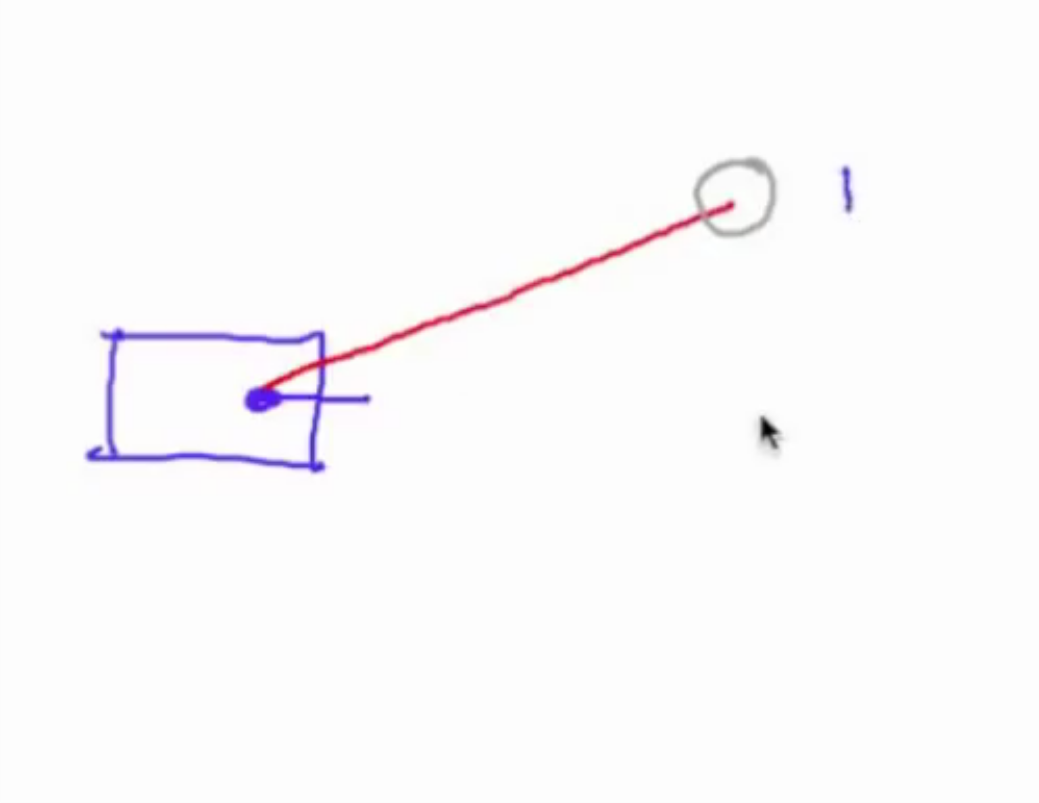
\includegraphics{../FIGURES/fig69}
\end{figure}

Later, if the robot does not report that it sees that landmark although
the landmark is within the visibility range of the scanner the algorithm
will decrement the counter associated to that landmark.

\begin{figure}[H]
\centering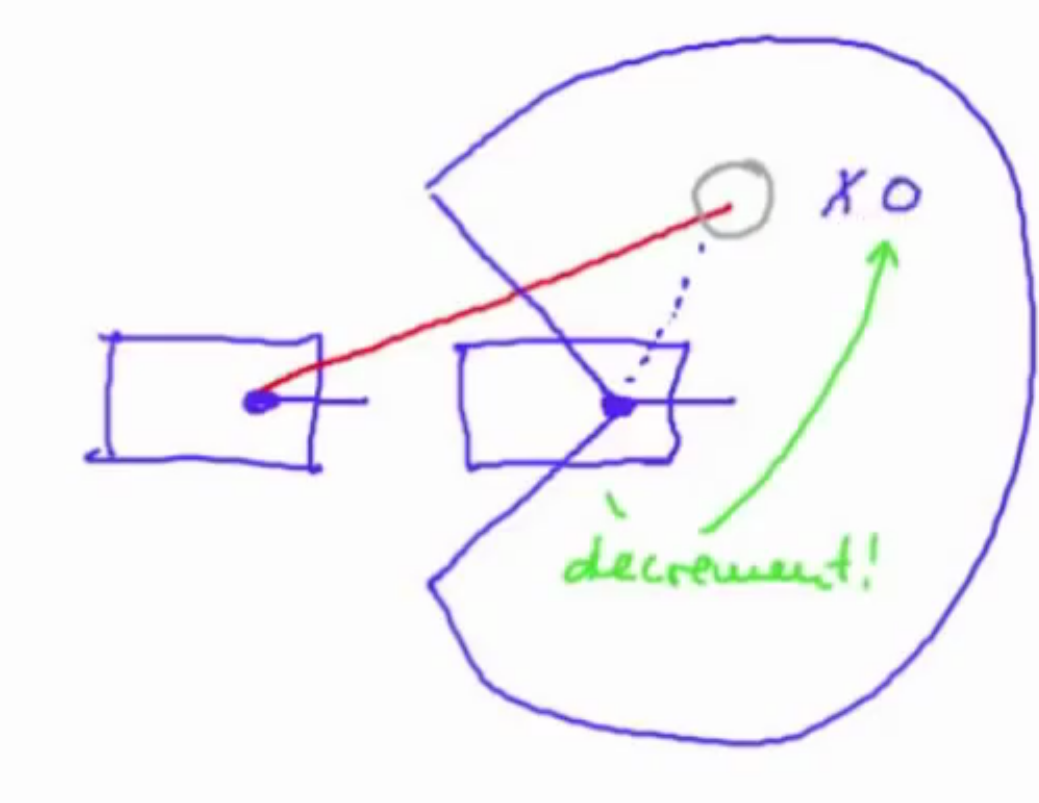
\includegraphics{../FIGURES/fig70}
\end{figure}

However, if the robot is somewhere where the landmark is not within
the visibility range of the laser scanner the algorithm will not decrement
the counter.

\begin{figure}[H]
\centering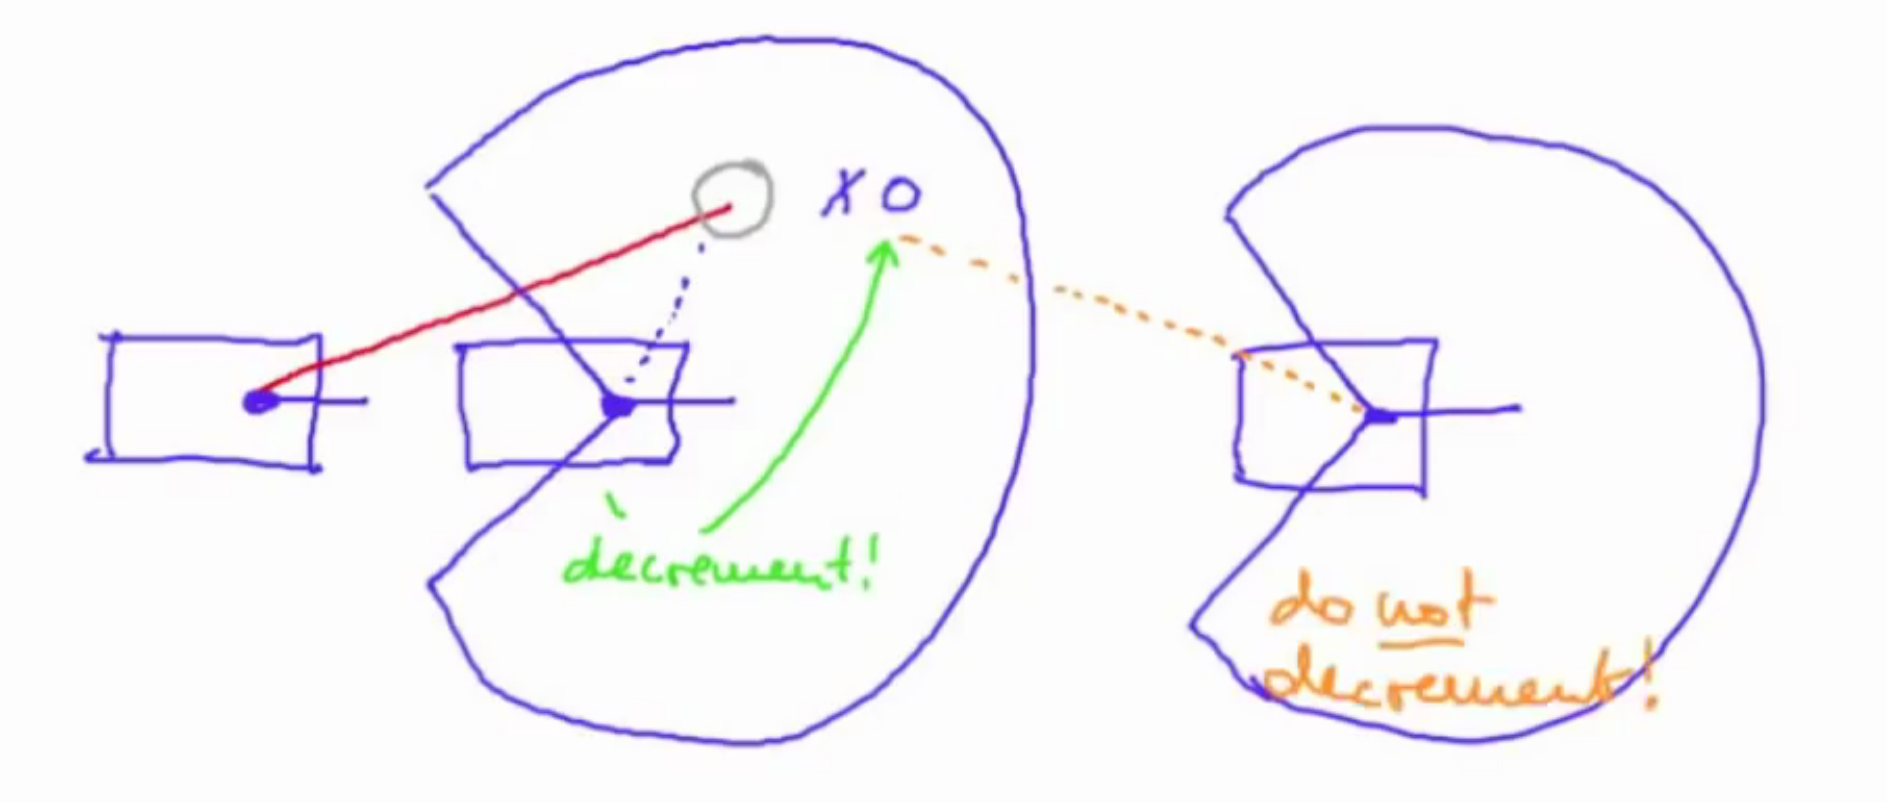
\includegraphics[scale=0.75]{../FIGURES/fig71}
\end{figure}

We will use in the algorithm a simplified method to decide whether
a landmark is within the visibility range of our LIDAR. We know the
minimum and maximum bearing angle of our scanner and we will consider
any existing landmark which has a bearing angle within that range
as being visible by our scanner.

\begin{figure}[H]
\centering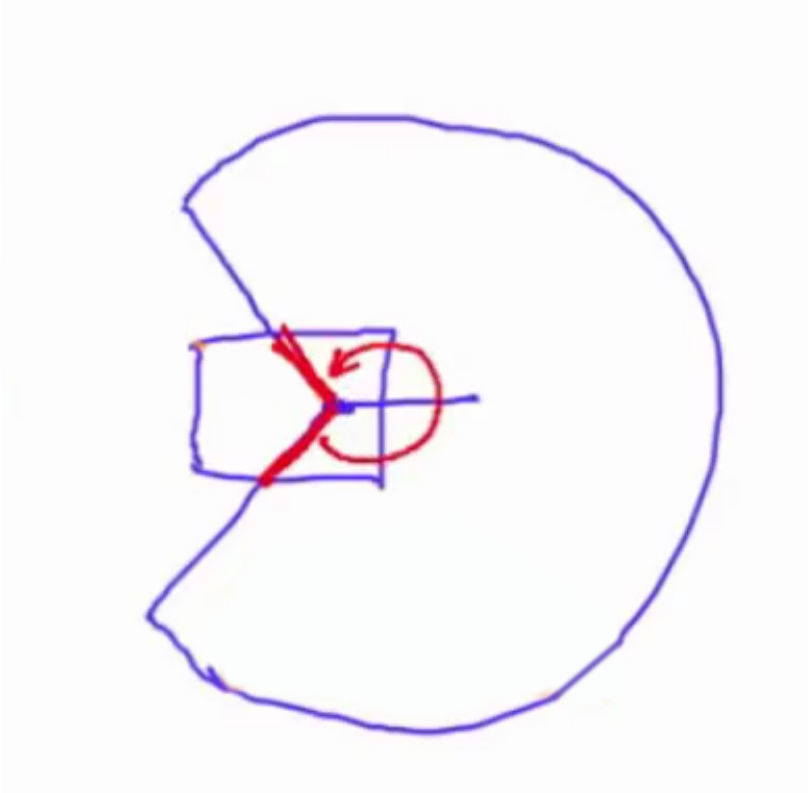
\includegraphics{../FIGURES/fig72}
\end{figure}

This over simplifies things a little bit. For example, as you know
our landmark detection works by detecting peaks in the scanner data
and so certainly if a landmark is for example at the beginning of
the scan measurement, like the landmark labeled as L in the next figure,
our method would fail to detect the landmark, nevertheless, our geometric
test would say that it is within the range of the laser scanner. Therefore,
for our simplified test we just don't care about this.

\begin{figure}[H]
\centering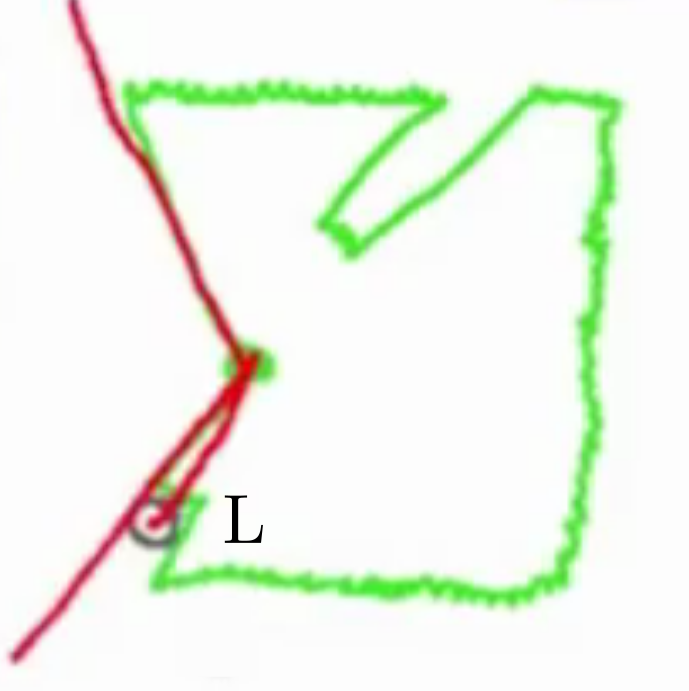
\includegraphics{../FIGURES/fig73}
\end{figure}

Also we don't handle occlusions correctly. For example if there are
two landmarks, L\textsubscript{1}and L\textsubscript{2}, settled
as in the next figure, the landmark detection process would detect
only the landmark L\textsubscript{1}but our visibility criterion
would consider both landmarks to be visible. Again, we don't care
about this case either.

\begin{figure}[H]
\centering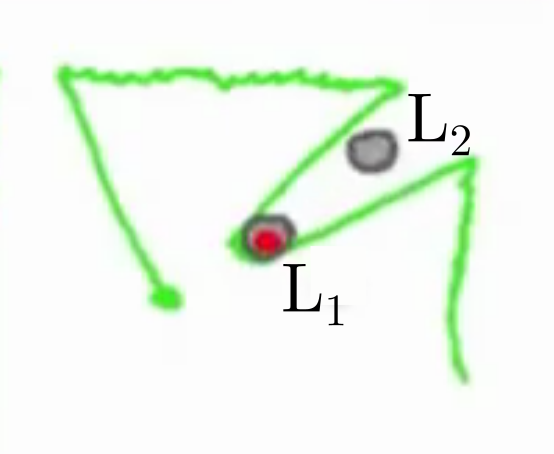
\includegraphics{../FIGURES/fig74}
\end{figure}

We will handle our landmark counter as follows. At a certain step
of our FAST-SLAM algorithm a certain particle has collected some landmarks,
so using the bearing angle criterion the algorithm will identify the
landmarks that are visible and decrement their counters by one whereas
it does not touch the counters of all landmarks which are not visible.

\begin{figure}[H]
\centering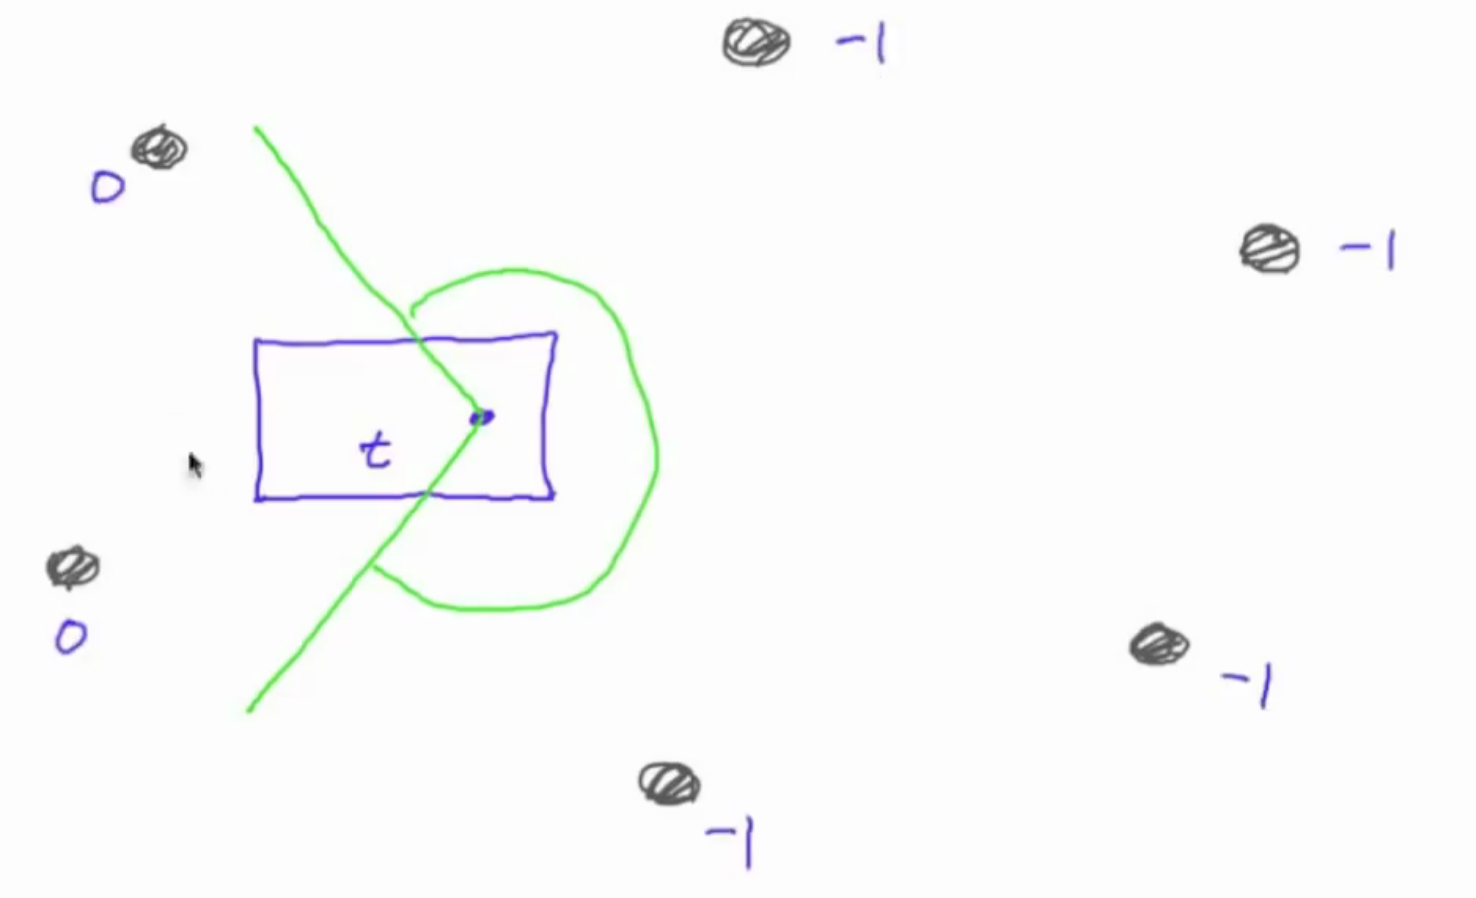
\includegraphics[scale=0.8]{../FIGURES/fig75}
\end{figure}

Now, the robot takes a scan and the algorithm extracts some observations.
The algorithm tries to assign these observations to the landmarks
using the maximum likelihood criterion.

Therefore, for those landmarks that can be associated with an observation
the algorithm will increment their counters by +2, so basically, for
these landmarks their associated counters have been effectively incremented
by +1 (-1 + 2 = +1).

For those landmarks that the algorithm does not touch anymore (but
they have been observed) their associated counters don't suffer any
change, so these associated counters have been effectively decremented
by -1.

For those landmarks that the algorithm observes for the first time
it will set an associated counter with value +1.

And finally, for those landmarks that are not visible, according to
our visibility criterion, their associated counters haven't suffered
any change in its value (+0).

After initializing the new landmarks the algorithm will loop over
all the landmarks of the particle and will test if the associated
counter's value for that landmark is smaller than 0. If the associated
counter's value for a landmark is smaller than 0 the landmark will
be deleted from the list of landmarks of that particle.

\begin{figure}[H]
\centering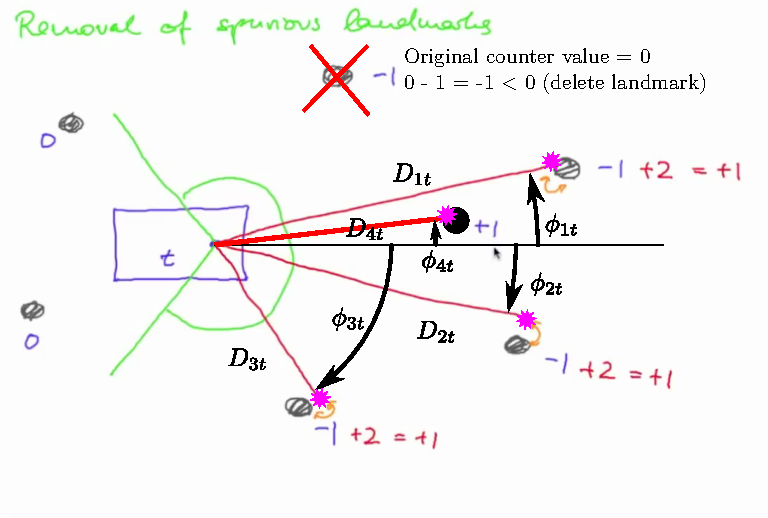
\includegraphics[scale=0.95]{../FIGURES/fig76}
\end{figure}

In the beginning the covariances of the landmarks get smaller and
then our particles travel along the trajectory. After a while we encounter
an undesired effect. The landmark 1, that has been observed multiple
times before, is now occluded by the landmark 4, so the value of the
counter associated with the landmark 1 is decremented and this results
in the landmark 1 being removed, at least for the particle that we
picked and whose landmarks are displayed here (remember that we are
displaying the closest particle, in the population of particles, to
the mean particle). Shortly after the landmark is observed again so
a new landmark is initialized (large uncertainty ellipse which gets
smaller subsequently).

\begin{figure}[H]
\centering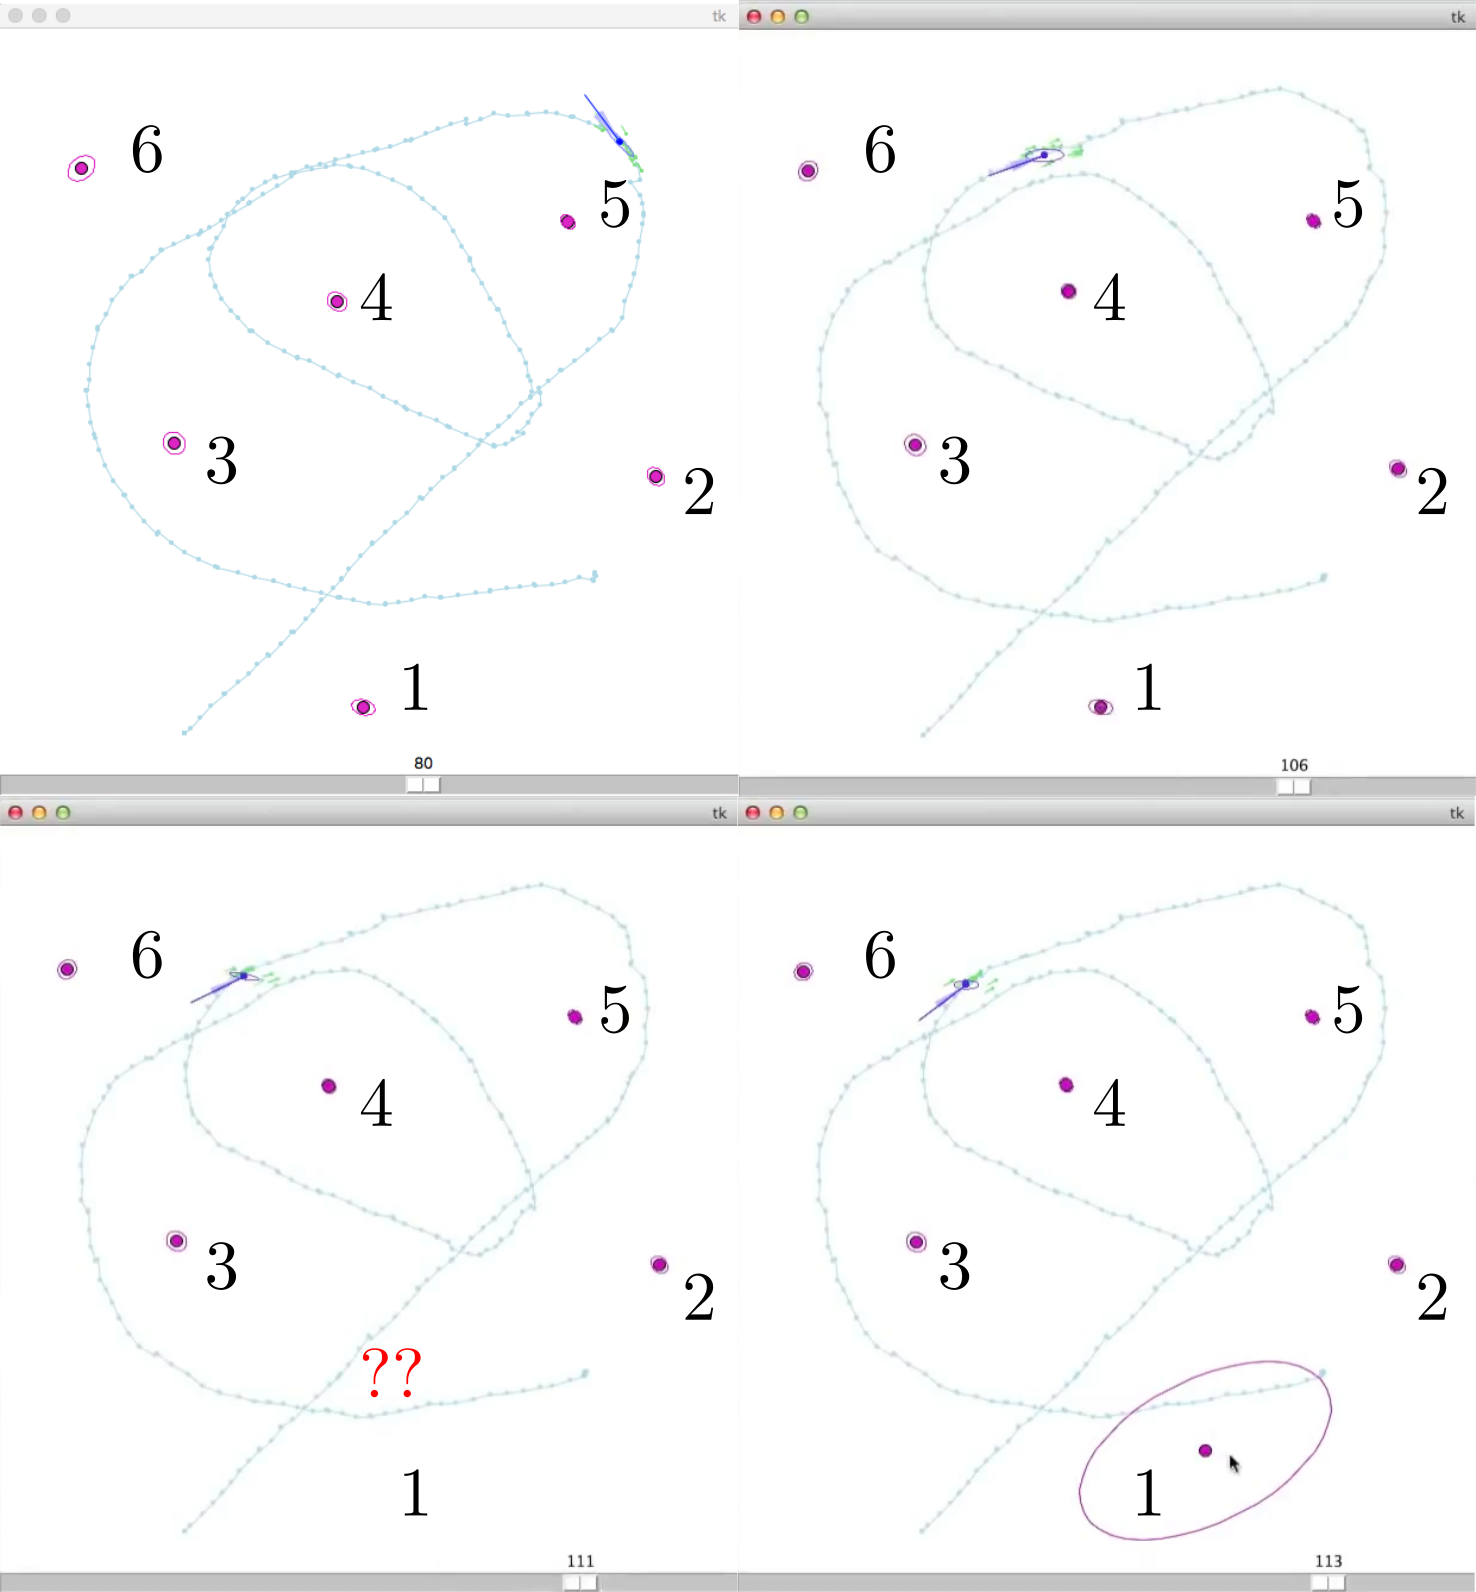
\includegraphics[scale=0.8]{../FIGURES/fig77}
\end{figure}

However note that our modification has solved our previous problem,
so even though sometimes spurious landmarks appear they are usually
removed shortly after so we get a pretty good result.

\begin{figure}[H]
\centering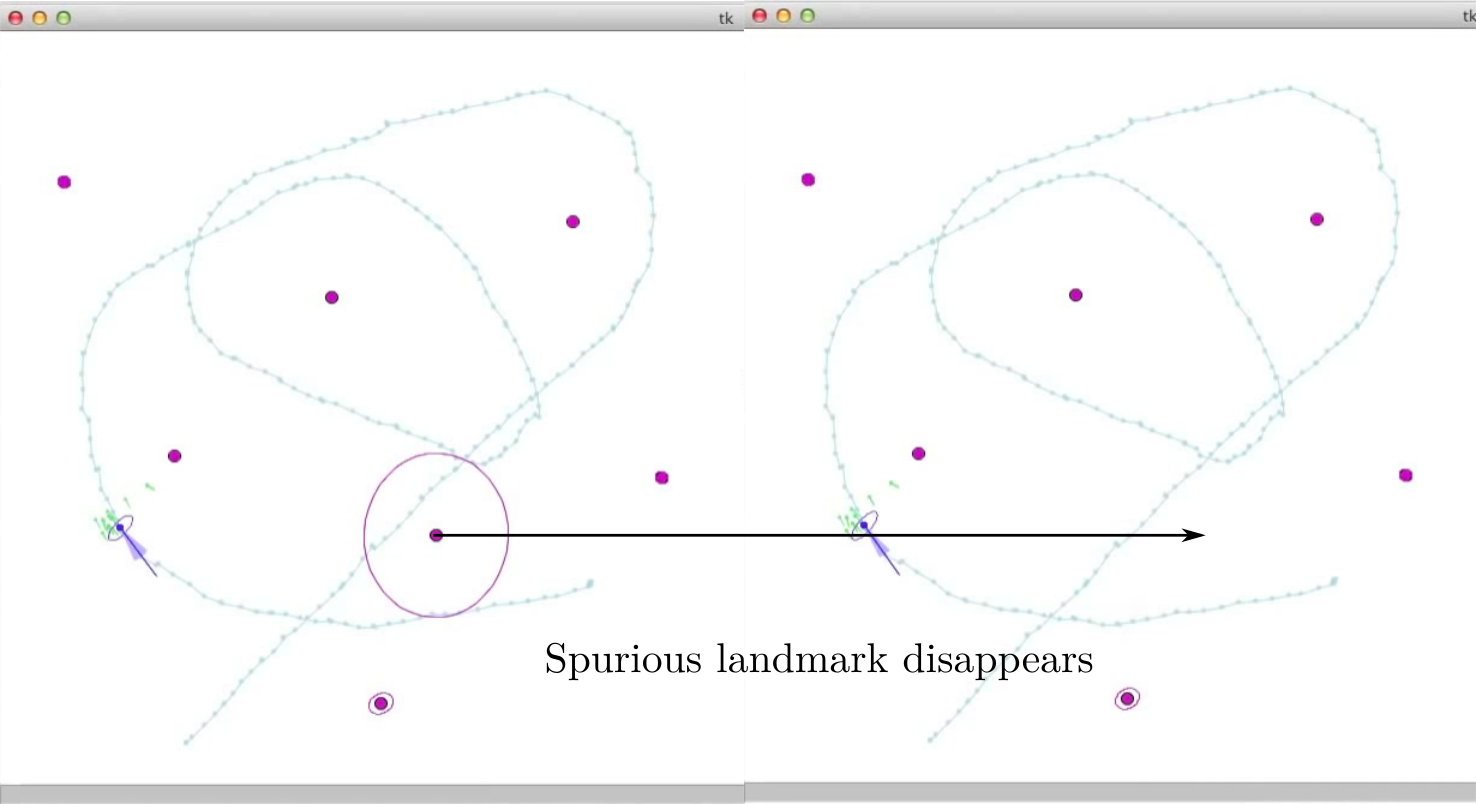
\includegraphics[scale=0.8]{../FIGURES/fig78}
\end{figure}

\begin{landscape}

\begin{figure}[H]
\centering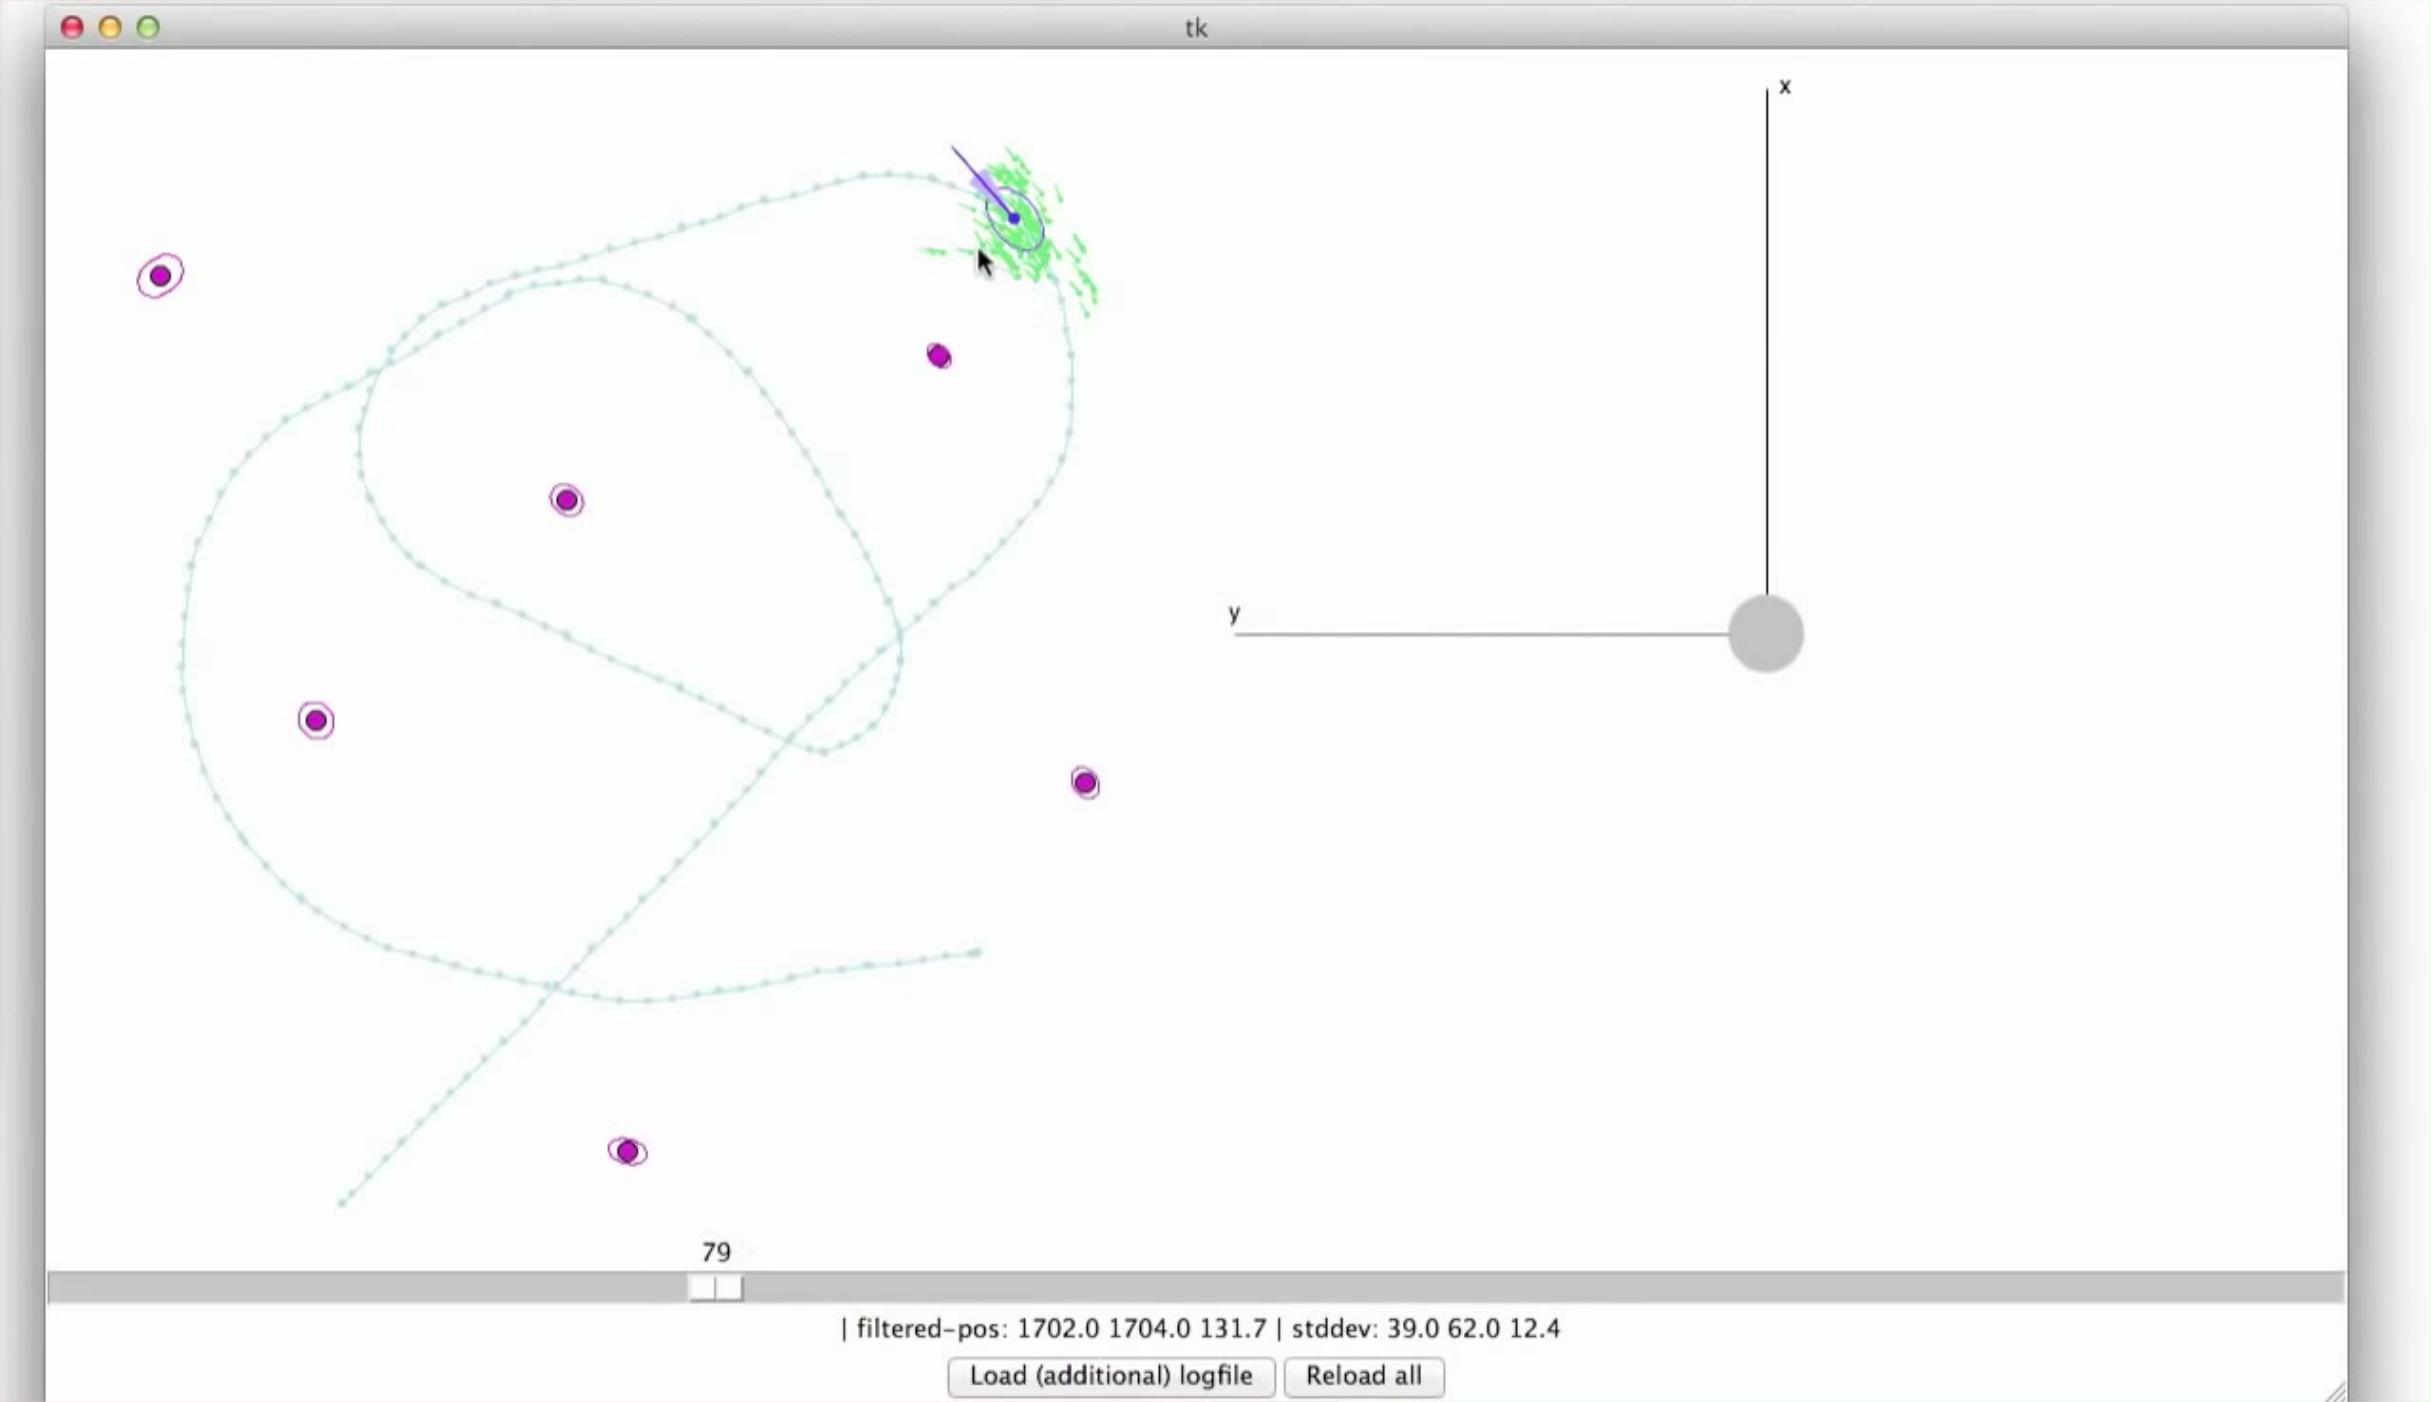
\includegraphics[scale=0.8]{../FIGURES/fig80}
\end{figure}

\end{landscape}
\end{document}
